\documentclass[tikz,border=5pt]{standalone}
\usepackage[T1]{fontenc}
\usepackage{lmodern,amsmath,amssymb}
\usetikzlibrary{arrows.meta,calc,positioning,fit,backgrounds,shapes.geometric,matrix,decorations.pathreplacing,patterns}
\definecolor{ink}{gray}{0.08}
\definecolor{wash}{gray}{0.965}
\definecolor{soft}{gray}{0.45}
\tikzset{box/.style={draw=ink,line width=.65pt,fill=white,align=center,inner sep=4pt,outer sep=0pt,font=\small},flow/.style={draw=ink,line width=.65pt,-{Latex[length=1.8mm,width=1.3mm]},rounded corners=2pt},annotation/.style={font=\scriptsize,text=soft,align=center},groupbox/.style={draw=soft,dashed,line width=.45pt,fill=wash}}
\begin{document}
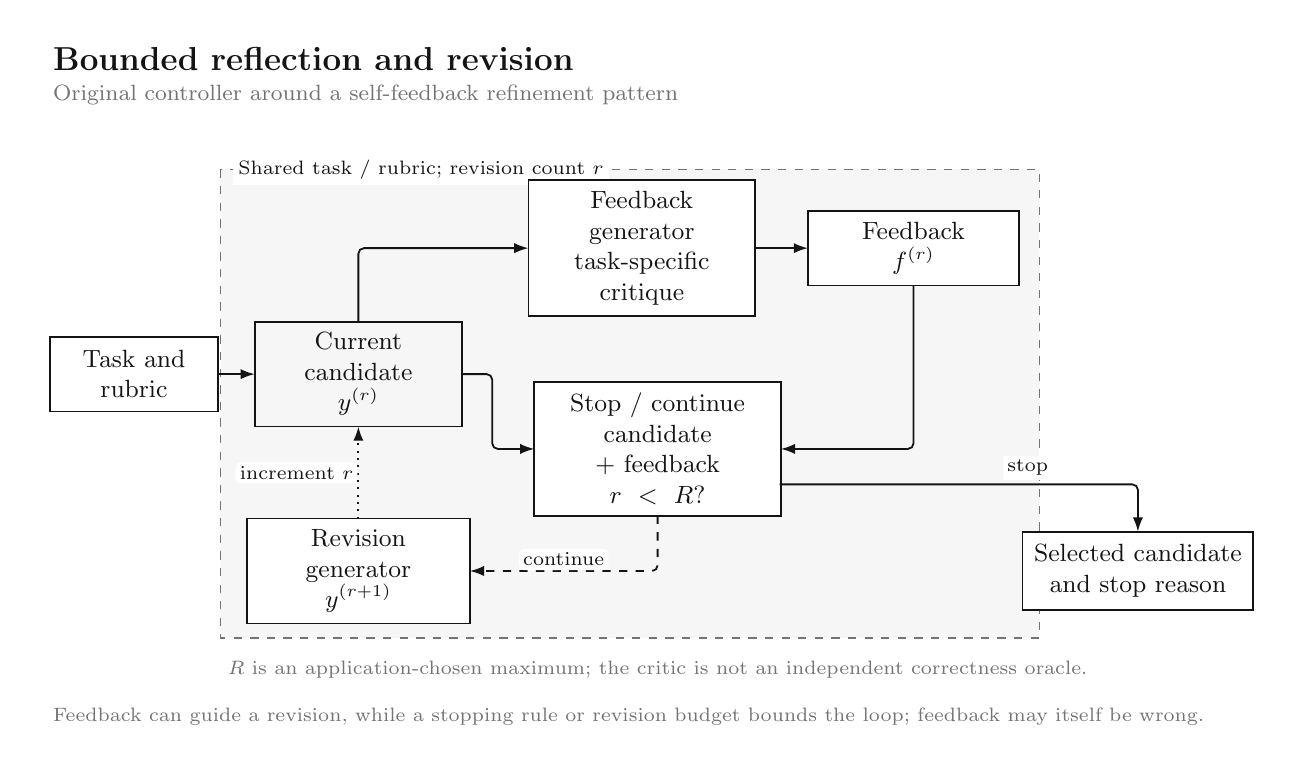
\begin{tikzpicture}[x=1cm,y=-1cm,font=\rmfamily,text=ink]

\path[use as bounding box] (0,0) rectangle (16,9);
\node[anchor=west,font=\large\bfseries] at (.2,.4) {Bounded reflection and revision};
\node[anchor=west,font=\footnotesize,text=soft] at (.2,.85) {Original controller around a self-feedback refinement pattern};
\begin{pgfonlayer}{background}
\draw[groupbox] (2.45,1.8) rectangle (12.850000000000001,7.75);
\node[anchor=west,font=\scriptsize,fill=white,inner sep=2pt] at (2.6,1.8) {Shared task / rubric; revision count $r$};
\end{pgfonlayer}
\node[box,minimum width=2.1cm,minimum height=0.95cm,text width=1.85cm] (input) at (1.35,4.4) {Task and rubric};
\node[box,fill=wash,minimum width=2.6cm,minimum height=1.1cm,text width=2.35cm] (draft) at (4.2,4.4) {Current candidate\\$y^{(r)}$};
\node[box,minimum width=2.85cm,minimum height=1.05cm,text width=2.6cm] (critic) at (7.8,2.8) {Feedback generator\\task-specific critique};
\node[box,minimum width=2.65cm,minimum height=0.95cm,text width=2.4cm] (feedback) at (11.25,2.8) {Feedback\\$f^{(r)}$};
\node[box,minimum width=3.1cm,minimum height=1.35cm,text width=2.85cm] (gate) at (8.0,5.35) {Stop / continue\\candidate + feedback\\$r < R$?};
\node[box,minimum width=2.8cm,minimum height=1.0cm,text width=2.55cm] (revise) at (4.2,6.9) {Revision generator\\$y^{(r+1)}$};
\node[box,minimum width=2.9cm,minimum height=1.0cm,text width=2.65cm] (output) at (14.1,6.9) {Selected candidate\\and stop reason};
\begin{pgfonlayer}{background}
\draw[flow] (input.east) -- (draft.west);
\draw[flow] (draft.north) -- (4.2,2.8) -- (critic.west);
\draw[flow] (critic.east) -- (feedback.west);
\draw[flow] (draft.east) -- (5.9,4.4) -- (5.9,5.35) -- (gate.west);
\draw[flow] (feedback.south) -- (11.25,5.35) -- (gate.east);
\draw[flow,dashed] (gate.south) -- (8.0,6.9) -- (revise.east) node[midway,above,fill=white,inner sep=1.5pt,font=\scriptsize] {continue};
\draw[flow,dotted] (revise.north) -- (draft.south) node[midway,left,fill=white,inner sep=1.5pt,font=\scriptsize] {increment $r$};
\end{pgfonlayer}
\draw[flow] (9.55,5.8) -- (14.1,5.8) -- (output.north);
\node[font=\scriptsize,fill=white,inner sep=1.5pt,anchor=south] at (12.7,5.75) {stop};
\node[annotation,anchor=center,text width=13cm] at (8.0,8.15) {$R$ is an application-chosen maximum; the critic is not an independent correctness oracle.};
\node[anchor=west,align=left,font=\scriptsize,text=soft,text width=15.6cm] at (.2,8.75) {Feedback can guide a revision, while a stopping rule or revision budget bounds the loop; feedback may itself be wrong.};
\end{tikzpicture}
\end{document}
